\section{Serial coordinate descent deconvolution}\label{cd}
In this section, we introduce the serial coordinate descent algorithm, which can replace CLEAN in the Major/Minor cycle architecture. We call this algorithm 'serial', because it minimizes exactly a single pixel in each iteration. Later in In Section \ref{pcdm} we introduce the parallel coordinate descent algorithm, which optimizes multiple pixels in a single iteration (multiple pixels in parallel).

In this project, the serial and parallel coordinate descent algorithm minimize the following convex objective function:

\begin{equation}\label{cd:deconv}
\underset{x}{minimize} \: \frac{1}{2} \left \| I_{dirty} - x * PSF \right \|_2^2 + \lambda ElasticNet(x)
\end{equation}

We want to find the minimum deconvolved image $x$, which is as close to the dirty image (remember the dirty image results from the visibilities, which get gridded and transformed to image space), but also has the smallest regularization penalty. The parameter $\lambda$ is a weight that either forces more or less regularization. It is either left to the user to define for each image, or can be estimated from the data \cite{miller1970least}. In this project, we leave $\lambda$ for the user to define. The objective function \eqref{cd:deconv} is convex, and we can use convex optimization methods to find a reconstructed image $x$. 

First, dive deeper into the elastic net regularization, and then continue with introducing the serial coordinate descent algorithm in Section \ref{cd:serial}. Although we call the algorithm 'serial', its implementation can use multiple processors in certain steps of the algorithm: For example updating a rectangle of pixels in the residual image can be trivially performed with multiple processors. We also created a GPU-accelerated and a distributed implementation of the serial coordinate descent algorithm. They can be found in the attachments, since both GPU-accelerated and distributed implementations were slower than the final CPU implementation of the parallel coordinate descent algorithm.

\subsection{Elastic net regularization} \label{cd:reg}
This regularization is a mixture between the L1 and L2 norm. The L1 norm is the absolute value of all pixels ($\left \| x \right \| = \sum_i \sum_j \left \| x_{ij} \right \|$), and the L2 norm is the squared sum of all pixels ($\left \| x \right \|_2 = \sum_i \sum_j \left \| x_{ij} \right \|^2$). The Figure \ref{cd:elastic} shows the effect of the L1 and L2 norm on a single star. The L1 norm forces the image to contain as few non-zero pixels as possible. It encodes our prior knowledge that the image will contain stars. The L2 regularization on the other hand "spreads" the single star across multiple pixels, which helps reconstructing extended emissions.

\begin{figure}[h]
	\centering
	\begin{subfigure}[b]{0.4\linewidth}
		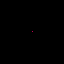
\includegraphics[width=\linewidth]{./chapters/03.CD/L1.png}
		\caption{Effect of the pure L1 norm ($\lambda$ = 1.0) on a single point source.}
		\label{cd:elastic:L1}
	\end{subfigure}
	\begin{subfigure}[b]{0.4\linewidth}
		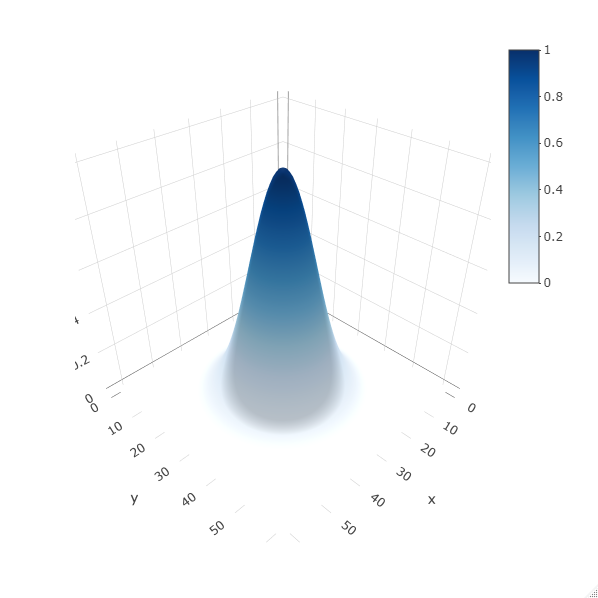
\includegraphics[width=\linewidth]{./chapters/03.CD/L2.png}
		\caption{Effect of the pure L2 norm ($\lambda$ = 1.0) on a single point source.}
		\label{cd:elastic:L2}
	\end{subfigure}
	
	\caption{Effect of the L1 and L2 Norm separately.}
	\label{cd:elastic}
\end{figure}

The L1 regularization alone models an image that consists of points sources. For extended emissions like hydrogen clouds, the L1 norm alone may force the algorithm to approximate the cloud with point sources. The L1 norm alone is not a good model for radio interferometric images that contain extended emissions. The L2 norm alone was already used in other image reconstruction algorithms in radio astronomy\cite{ferrari2014distributed}, with the downside that the resulting image will not be sparse. I.e. all pixels in the reconstruction will be non-zero, even though some of them only contain noise. 

Elastic net mixes the L1 and L2 norm together, becoming "sparsifying L2 norm". It retains the sparsifying property of the L1 norm, while also keeping extended emissions in the image. Formally, elastic net regularization is defined as the following regularization function:

\begin{equation}\label{cd:elastic:formula}
ElasticNet(x, \alpha) = \: \alpha \left \|x \right \|_1 + \frac{1-\alpha}{2}  \left \|x \right \|_2
\end{equation}

The parameter $\alpha$ is between 0 and 1, and mixes the two norms together. A value of 1 leads to L1 regularization only, and a value of 0 leads to L2 only. The elastic net regularization has two properties, which are relevant later for the serial coordinate descent algorithm: It is separable, and has a proximal operator.

Separability means that we can calculate the elastic net regularization penalty independently for each pixel. We arrive at the same result if we evaluate \eqref{cd:elastic:formula} for each pixel and sum up the results, or if we evaluate \eqref{cd:elastic:formula} for the whole image. This is an important property when one tries to minimize the objective function \eqref{cd:deconv} used in this project. We can minimize a single pixel at a time, and do not need to account for the whole neighborhood.

The proximal operator of elastic net allows us to minimize the regularization penalty. Notice that the elastic net regularization \eqref{cd:elastic:formula} is not differentiable (the L1 norm is not continuous). We cannot calculate a gradient. However, it has a proximal operator defined:

\begin{equation}\label{cd:elastic:proximal}
ElasticNetProximal(x, \lambda ,\alpha) = \: \frac{max(x - \lambda \alpha, 0)}{1+\lambda(1 - \alpha)}
\end{equation}

The proximal operator allows us to minimize the deconvolution problem with an elastic net regularization. We can calculate the gradient of the data term of \eqref{cd:deconv}, which is differentiable. Then, we apply the proximal operator on the gradients. Descending these modified gradients minimizes the objective function \eqref{cd:deconv}. The proximal operator of elastic net can be applied on the gradient of each pixel independently. Neighboring pixels do not influence the regularization.

A side note on the proximal operator used in this project \eqref{cd:elastic:proximal}: The numerator always clamps negative pixels to zero. This is a conscious design decision. In radio astronomy, it is usual to constrain the reconstruction to be non-negative (because we cannot receive negative radio emissions from any direction). It is widely used in radio astronomy image reconstruction and may lead to improved reconstruction quality \cite{mcewen2011compressed}.


\subsection{Serial coordinate descent algorithm}\label{cd:serial}
Our serial coordinate descent deconvolution algorithm minimizes the deconvolution objective \eqref{cd:deconv} for a single pixel at each iteration. Each iteration consists of two steps. Step 1: Find the best pixel to optimize. Step 2: Calculate the gradient for this pixel, apply the elastic net proximal operator, and take a descent step for the single pixel. The algorithm iterates over all pixel multiple times to converge to a reconstructed image.

We demonstrate the serial deconvolution algorithm with the help of a simulated MeerKAT reconstruction problem of two point sources. Figure \ref{cd:serial:aid:dirty} shows the dirty image of two point sources, and Figure \ref{cd:serial:aid:psf} the $PSF$. The deconvolved image with elastic net regularization is shown in Figure \ref{cd:serial:aid:elastic}. I.e. Figure \ref{cd:serial:aid:elastic} is the optimum $x$ of the objective function \eqref{cd:deconv}.

\begin{figure}[h]
	\centering
	\begin{subfigure}[b]{0.3\linewidth}
		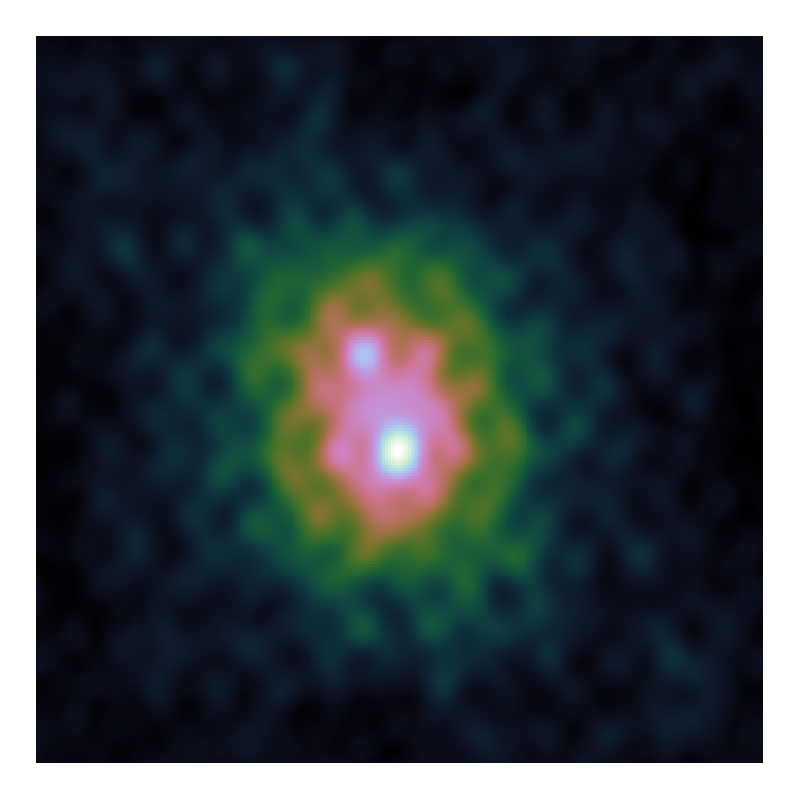
\includegraphics[width=\linewidth, clip, trim= 0.25in 0.25in 0.25in 0.25in]{./chapters/03.cd/simulated/dirty.png}
		\caption{Dirty Image.}
		\label{cd:serial:aid:dirty}
	\end{subfigure}
	\begin{subfigure}[b]{0.3\linewidth}
		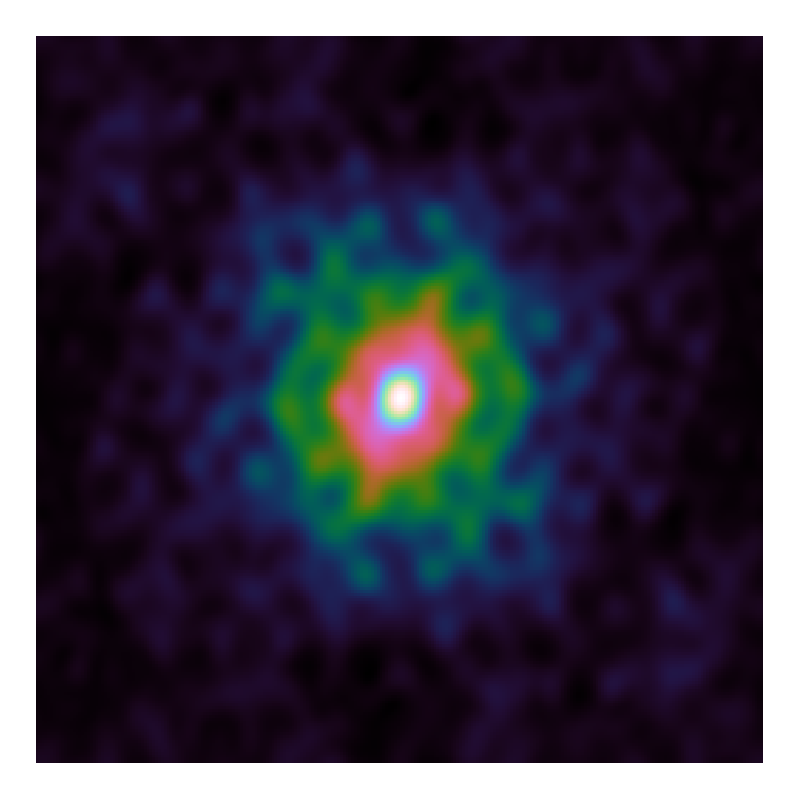
\includegraphics[width=\linewidth, clip, trim= 0.25in 0.25in 0.25in 0.25in]{./chapters/03.cd/simulated/psf.png}
		\caption{Point Spread Function.}
		\label{cd:serial:aid:psf}
	\end{subfigure}
	\begin{subfigure}[b]{0.3\linewidth}
		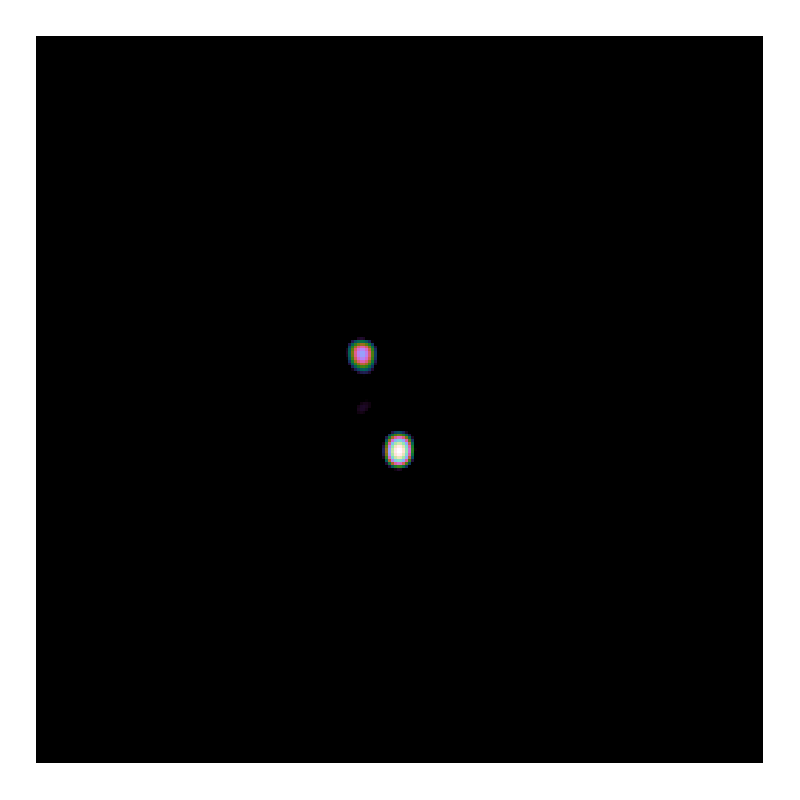
\includegraphics[width=\linewidth, clip, trim= 0.25in 0.25in 0.25in 0.25in]{./chapters/03.cd/simulated/elasticNet.png}
		\caption{Elastic net reconstruction}
		\label{cd:serial:aid:elastic}
	\end{subfigure}

	\caption{Example problem with two point sources.}
	\label{cd:serial:aid:figure}
\end{figure}

\subsubsection{Step 1: Choosing single a pixel}
For coordinate descent methods, there are several strategies to choose a single coordinate (pixel). Our serial coordinate descent algorithm uses a greedy strategy. In the first step, we iterate over all pixels and calculate its gradient. We select the pixel which has the largest gradient magnitude. In each iteration, the greedy strategy chooses the pixel, which results in the largest decrease of our objective function \eqref{cd:deconv}. There are two other strategies that are often used in coordinate descent methods: Random and Cyclic.
%with the maximum possible difference in this iteration

A random strategy chooses, as the name implies, a pixel at random. Usually, the pixels are chosen from a uniform distribution. The random strategy leads to cheaper iteration compared to the greedy strategy, because we do not check the gradient of each pixel.

A cyclic strategy iterates over a subset of pixels until the subset converges. It then chooses another subset. Each iteration of the cyclic strategy is also cheaper than the greedy strategy. 

For our image deconvolution problem, we choose the greedy strategy. Even though it is more expensive, it tends to be faster to converge on the deconvolution problem in radio astronomy. Our reconstructed image is sparse, meaning most pixels in the image will be zero. The greedy strategy tends to choose pixels which will be non-zero in the final reconstructed image. The random or cyclic strategy will set pixels to a non-zero value, which will eventually become zero in the final image. For the deconvolution problem, removing pixels from an intermediate solution seems to slow down the time to converge. We will discuss the different selection strategies in detail for the parallel coordinate descent methods.


\subsubsection{Step 2: Optimizing a single pixel}
At this point, the greedy strategy has selected a pixel at a specific location to minimize. The serial coordinate descent algorithm minimizes a single pixel at each iteration, and our deconvolution objective \eqref{cd:deconv} is reduced from a large number of dimensions (pixels), to a one dimensional problem\footnote{The reason why this reduces nicely to one dimension is the elastic net regularization is separable. I.e. the regularization can be calculated independently of the surrounding pixels.}:  

\begin{equation}\label{cd:serial:step2:onedim}
\underset{x}{minimize} \: \frac{1}{2} \left \| I_{dirty} - x_{location} * PSF \right \|_2^2 + \lambda ElasticNet(x_{location})
\end{equation}

Optimizing the one dimensional problem \eqref{cd:serial:step2:onedim} is a lot simpler. In essence, we calculate the gradient for the pixel at the selected location, and apply the proximal operator of elastic net. First, let us look at how the gradient is calculated and ignore the regularization. The gradient arises from the data term of the one dimensional objective \eqref{cd:serial:step2:onedim} ($\left \| I_{dirty} - x_{location} * PSF \right \|_2^2$). After simplifying the partial derivative, we arrive at the calculation:

\begin{equation}\label{cd:serial:step2:gradient}
\begin{split}
residuals &= I_{dirty} - x * PSF \\
gradient_{location} &= \langle residuals, PSF_{location} \rangle \\
Lipschitz_{location} &= \langle PSF_{location}, PSF_{location} \rangle \\
pixel_{opt} &= \frac{gradient_{location}}{Lipschitz_{location}}
\end{split}
\end{equation}

First, we calculate the residuals by convolving the current solution $x$ with the $PSF$. Then, the gradient for the selected pixel location is the inner product (element-wise multiplication followed by a sum over all elements) of the residuals and the $PSF$, shifted at the current location. The next step is to calculate the Lipschitz constant at the current location. Finally, we arrive at the optimal pixel value by dividing the gradient with the Lipschitz constant (The optimal deconvolved pixel value, ignoring the regularization).

The Lipschitz constant can be thought of as the step size. It defines how far we can descend towards the direction of the gradient. The Lipschitz constant describes how fast a function $f(x)$ changes with $x$. If $f(x)$ changes slowly, we can descend larger distances along the gradient without the fear for divergence. The Lipschitz constant can be looked at as a data-defined step size.

An interesting point is that the update rule $pixel_{opt} = \frac{gradient_{location}}{Lipschitz_{location}}$ finds the optimal pixel value, if the pixel is independent. Remember that our objective function is convex. The data term of our one dimensional objective \eqref{cd:serial:step2:onedim} actually forms a parabola, with the parameters: $x^2 \langle PSF, PSF \rangle - 2x \langle resdiuals, PSF_{location}\rangle + c$. Calculating the optimum of the parabola $\frac{-b}{2a}$, is identical to calculating the gradient update \eqref{cd:serial:step2:gradient}. Note that $b = -2 gradient_{location}$ and $a = Lipschitz_{location}$, and both the minimum of the parabola $\frac{-b}{2a}$ and the update rule based on partial derivatives \eqref{cd:serial:step2:gradient} are identical.

This means if our reconstruction problem has point sources which are far away, such that their $PSF$s do not overlap, then the update rule finds the optimal value for each point source with one iteration. But when the $PSF$s overlap as in our example problem, shown in Figure \ref{cd:serial:aid:figure}, then we need several iterations to sort out the correlated pixels. The serial coordinate descent algorithm needs to iterate over the same pixel several times until it converges.

\textbf{Including the elastic net regularization}\\
So far, we ignored the regularization. We can calculate the optimal pixel value without elastic net regularization. The last step is to combine the proximal operator of the elastic net regularization \eqref{cd:elastic:proximal} with the gradient calculation, and we arrive at the following update step:

\begin{equation} \label{cd:serial:step2:update}
pixel_{opt} = \frac{max(gradient_{location} - \lambda\alpha, 0)}{Lipschitz_{location} + (1 - \alpha)\lambda}
\end{equation}

This update rule now finds the optimal pixel value with elastic net regularization. If the $PSF$s do not overlap, we still only need one iteration per source.

Note that our algorithm calculates the gradient for a single pixel in each iteration. This may raise the question: What exactly is the difference between gradient- and coordinate descent? The difference is that gradient descent optimizes all pixels in each iteration, while coordinate descent optimizes (generally) a single pixel at a time\footnote{There are block coordinate descent methods that optimize a block of coordinates at each iteration. They are also discussed together with parallel coordinate descent methods in Section \ref{pcdm}}. Also, Coordinate descent methods are not bound to use the gradient. It could use a line search approach, where we try different values and decide on the one leading to the lowest objective value.

Optimizing a single pixel at a time can be an advantage for the deconvolution problem. There is a trade-off between descending a single pixel at a time, or a group of pixels: A gradient based algorithm can change a large value of a single pixel, or a smaller value for a group of pixels without the danger of diverging. The more pixels are changed in every iteration, the smaller the change can be for each pixel. In the deconvolution problem, large parts of the reconstructed image will be zero. We want the optimization algorithm to focus its changes on pixels, which are non-zero in the final reconstruction.

Now we put together our serial coordinate descent algorithm, and show where the bottleneck lies. In each iteration, the serial coordinate descent algorithm selects the pixel with the maximum gradient magnitude, and optimizes the selected pixel with the update rule \eqref{cd:serial:step2:update}.

\begin{lstlisting}
dirty = IFFT(GridVisibilities(visibilities))
residuals = dirty

x = new Array
objectiveValue = 0.5* Sum(residuals * residuals) + ElasticNet(x)

diff = 0
do 
	oldObjectiveValue = objectiveValue
	
	//Step 1: Search pixel
	pixelLocation = GreedyStrategy(residuals, PSF)
	oldValue = x[pixelLocation]
	shiftedPSF = Shift(PSF, pixelLocation)
	
	//Step 2: Optimize pixel
	gradient = Sum(residuals * shiftedPSF)
	lipschitz = Sum(shiftedPSF * shiftedPSF)
	tmp = gradient + oldValue * lipschitz 
	optimalValue = Max(tmp - lambda*alpha) / (lipschitz + (1 - alpha)*lambda)
	x[pixelLocation] = optimalValue

	//housekeeping
	diff = newValue - oldValue
	residuals = residuals - shiftedPSF * (optimalValue - oldValue)
while epsilon < Abs(diff) 
\end{lstlisting}

The actual update step is cheap to compute. We are only dealing with four one dimensional variables. The expensive calculations are the inner products: The gradient calculation, the Lipschitz constant and the objective value. The residuals and $PSF$ generally contain millions of pixels. Calculating the inner product of those becomes expensive. 

Also note that the greedy strategy needs to calculate the gradient for each pixel. As it is, the greedy strategy has a quadratic runtime complexity. 

\subsection{Efficient implementation}\label{cd:efficient}
Because coordinate descent methods only optimize a single pixel at a time, they generally need a large number of iterations to converge compared to other methods. But when each iteration is cheap to compute, coordinate descent methods can converge to a result in less time than competing methods\cite{nesterov2012efficiency, nesterov2013gradient}. We now discuss the efficient implementation.

The bottleneck of the serial coordinate descent algorithm are all the inner products that need to be calculated in each iteration. In each iteration, we need to know the gradient for every pixel, and the Lipschitz constant of the current pixel. Luckily, we can cache a map of gradients, where we save the gradient for every pixel and skip all of the inner products associated with the gradient. The Lipschitz constants are, as the name implies, constant for the whole deconvolution. They can be pre-calculated and cached for each pixel. The efficient calculation of Lipschitz constants can be found in the Attachments. We can greatly reduce the runtime cost for each iteration.


\subsubsection{Edge handling of the convolution}
As the reader is probably aware, there are several ways to define the convolution in image processing, depending on how we handle the edges on the image. Two possibilities are relevant for radio interferometric image reconstruction: Circular and zero padded.

\begin{figure}[h]
	\centering
	\begin{subfigure}[b]{0.3\linewidth}
		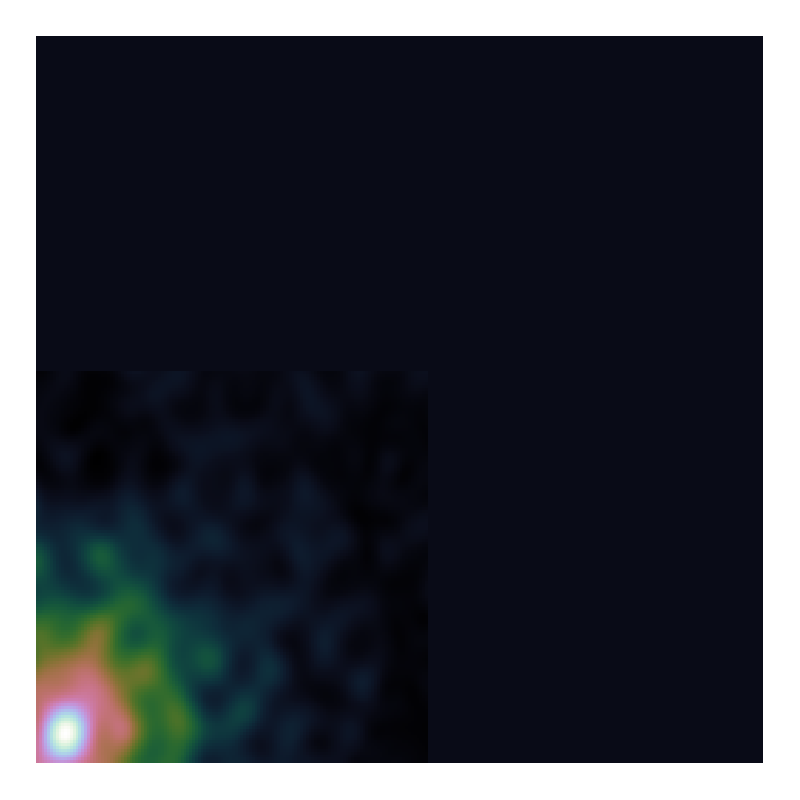
\includegraphics[width=\linewidth, clip, trim= 0.25in 0.25in 0.25in 0.25in]{./chapters/03.cd/simulated/psfZeroPadding.png}
		\caption{Zero padded convolution.}
		\label{cd:efficient:convolution:padded}
	\end{subfigure}
	\begin{subfigure}[b]{0.3\linewidth}
		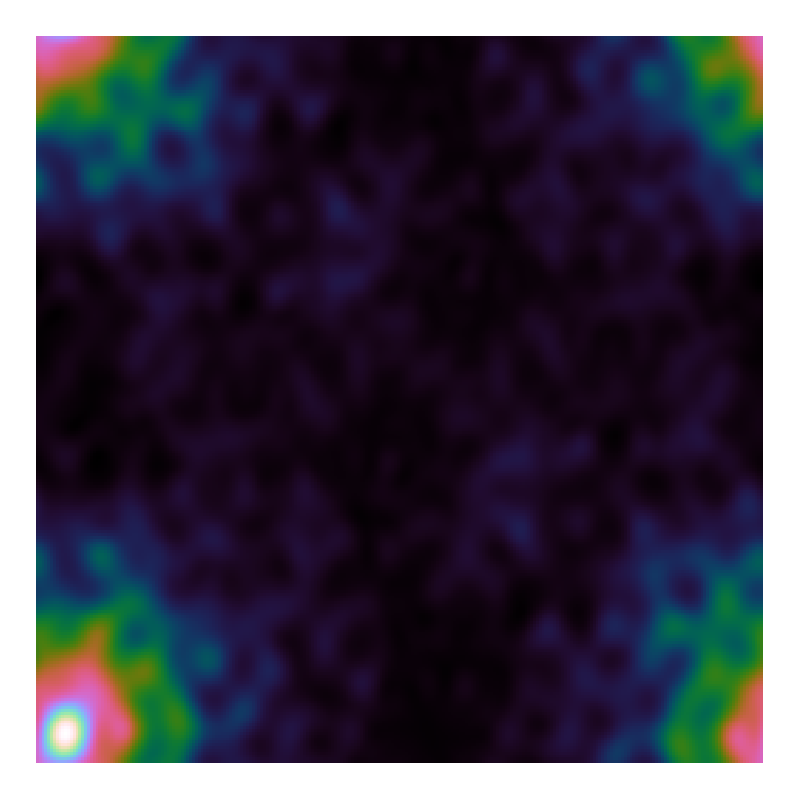
\includegraphics[width=\linewidth, clip, trim= 0.25in 0.25in 0.25in 0.25in]{./chapters/03.cd/simulated/psfCircular.png}
		\caption{Circular convolution.}
		\label{cd:efficient:convolution:circular}
	\end{subfigure}
	\caption{Comparison of the two convolution schemes.}
	\label{cd:efficient:convolution:figure}
\end{figure}

Circular convolution assumes the image "wraps" around itself. If we travel over the right edge of the image, we arrive at the left edge. The convolution in Fourier space is circular. Remember: A convonlution in image space is a multiplication in Fourier space, and vice versa. When we convolve the reconstructed image $x$ with the $PSF$ using circular convolution, then non-zero pixels at the right edge of the image "shine" over to the left edge. This is physically impossible.

Zero padding assumes that after the edge, the image is zero. Non-zero pixels at the right edges of the image do not influence the left edge after convolution. This is the physically plausible solution. However, the zero padded convolution is more expensive to calculate. We either have to calculate the convolution in image space, which is too expensive for large kernels, or apply the FFT on a zero-padded image. Either way, it is more expensive than the circular convolution.

In designing a deconvolution algorithm, we have the choice between the circular and the zero-padded convolution scheme. Circular convolution is more efficient to calculate, while zero-padded convolution is closer to the reality. Both choices are possible. Some implementations leave this choice to the user \cite{kenyon2019pymoresane}. We decide on using the zero-padded convolution. This choice influences how we calculate the Lipschitz and gradients efficiently.


\subsubsection{Using a map of gradients}
For an efficient greedy strategy, we need to know the gradient for each pixel.  We show how to calculate the initial map of gradients efficiently with the FFT, and how to update it directly after a change in the reconstructed image $x$. As we will see, we can use a map of gradients and drop the residual image from the algorithm. The gradient map implicitly contains the information of the residuals.

\textbf{Efficient initialization }\\
Calculating the gradient for each pixel results again in a quadratic runtime. We need to calculate $\langle residuals, PSF_{location} \rangle$ for every pixel. But we can use the FFT to efficiently calculate the map of gradients in time. Note that the inner product is actually a correlation: We correlate the $PSF$ with the residuals. The correlation and the convolution are related. The convolution is simply a correlation with a flipped kernel. This means we can use the $FFT$ to efficiently calculate the correlation of the residuals and the $PSF$:

\begin{equation}\label{cd:efficient:gradients:correlation}
\begin{split}
psfFlipped &= FlipUD(FlipLR(PSF)) \\
gradients &= iFFT(FFT(residuals) * FFT(psfFlipped))
\end{split}
\end{equation}

A convolution in image space is a multiplication in Fourier space. This fact can also be exploited for the correlation by flipping the $PSF$. Since the FFT takes linearithmic time $O(n log n)$ to compute, the overall operation also takes us linearithmic time. The operation is shown in Figure \ref{cd:efficient:gradients:figure}.

\begin{figure}[h]
	\centering
	\begin{subfigure}[b]{0.3\linewidth}
		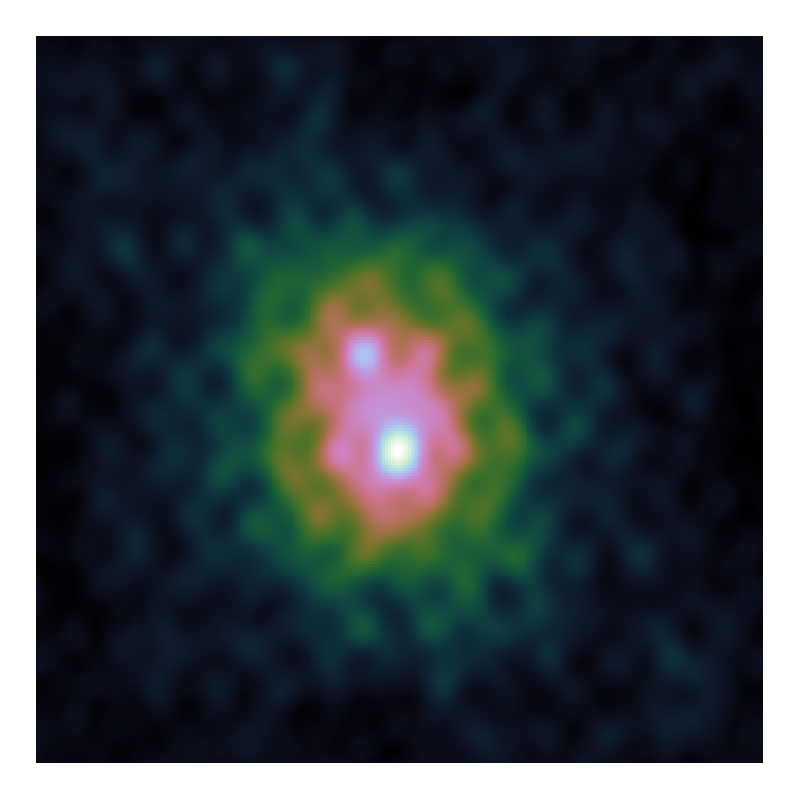
\includegraphics[width=\linewidth, clip, trim= 0.25in 0.25in 0.25in 0.25in]{./chapters/03.cd/simulated/dirty.png}
		\caption{Dirty Image.}
		\label{cd:efficient:gradients:dirty}
	\end{subfigure}
	\begin{subfigure}[b]{0.3\linewidth}
		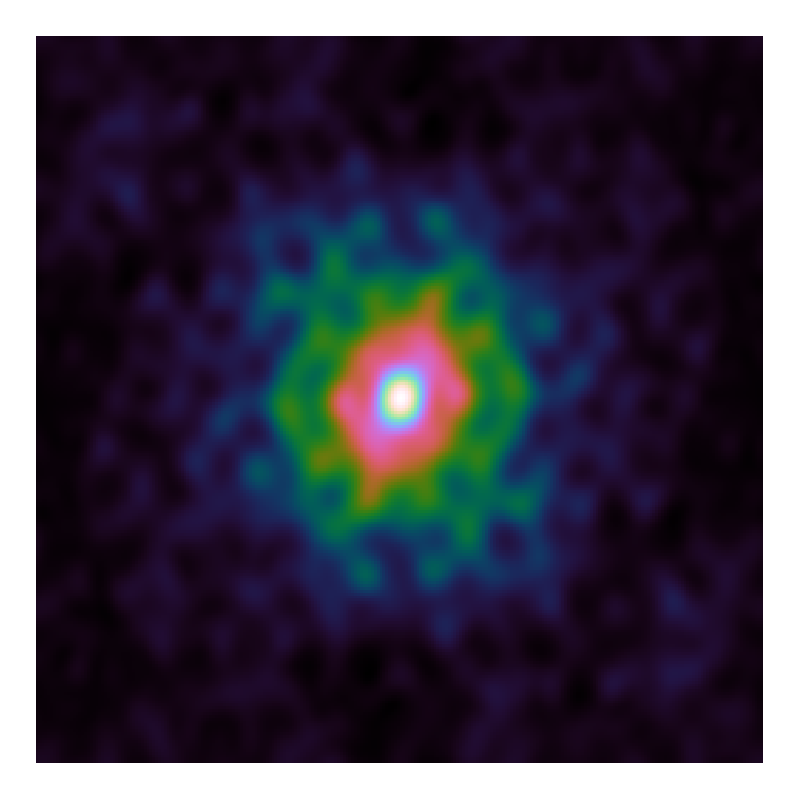
\includegraphics[width=\linewidth, clip, trim= 0.25in 0.25in 0.25in 0.25in]{./chapters/03.cd/simulated/psf.png}
		\caption{Point Spread Function.}
		\label{cd:efficient:gradients:psf}
	\end{subfigure}
	\begin{subfigure}[b]{0.3\linewidth}
		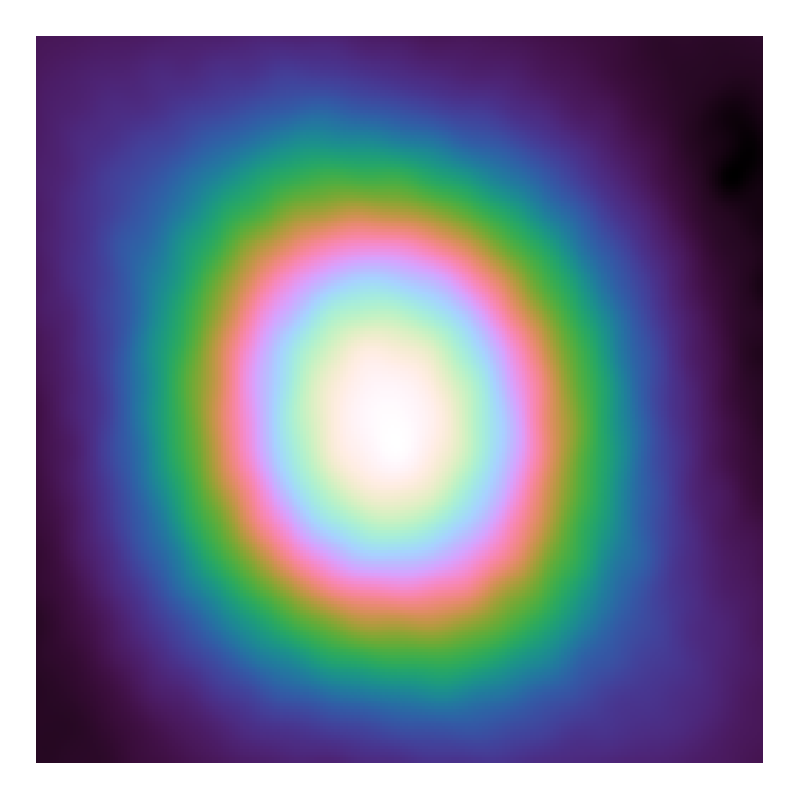
\includegraphics[width=\linewidth, clip, trim= 0.25in 0.25in 0.25in 0.25in]{./chapters/03.cd/simulated/gradients.png}
		\caption{Gradient map.}
		\label{cd:efficient:gradients:gradients}
	\end{subfigure}
	
	\caption{Example of the gradient calculation.}
	\label{cd:efficient:gradients:figure}
\end{figure}


\textbf{Direct update of gradient map}\\
Thanks to the FFT, we can efficiently calculate the map of gradients at the start of the serial coordinate descent algorithm. After we update a pixel in the reconstruction $x$, the map changes. We could repeat the correlation in the Fourier space from equation \eqref{cd:efficient:gradients:correlation} at each iteration. But this is wasteful. We can update the map of gradients directly.

Note that if we add a pixel in the reconstruction $x$, we subtract the $PSF$ (multiplied with the pixel value) from the specific location in the residuals. The gradient map is then calculated by again correlating the $PSF$ with the residuals. We update the residuals by subtracting the $PSF$ at the correct location. And we update the gradient map by subtracting the $PSF$ correlated with itself at the correct position ($PSF \star PSF$). In our simulated example, the $PSF$ and the gradient update map is shown in Figure \ref{cd:efficient:update:psf}.
\begin{figure}[!h]
	\centering
	\begin{subfigure}[b]{0.3\linewidth}
		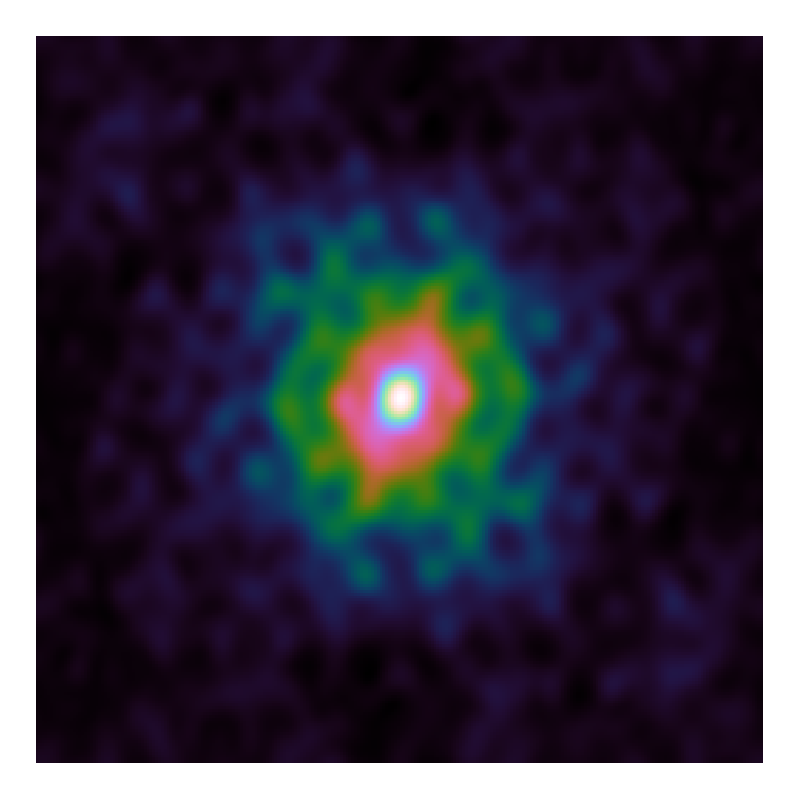
\includegraphics[width=\linewidth, clip, trim= 0.25in 0.25in 0.25in 0.25in]{./chapters/03.cd/simulated/psf.png}
		\caption{Point Spread Function.}
		\label{cd:efficient:update:dirty}
	\end{subfigure}
	\begin{subfigure}[b]{0.3\linewidth}
		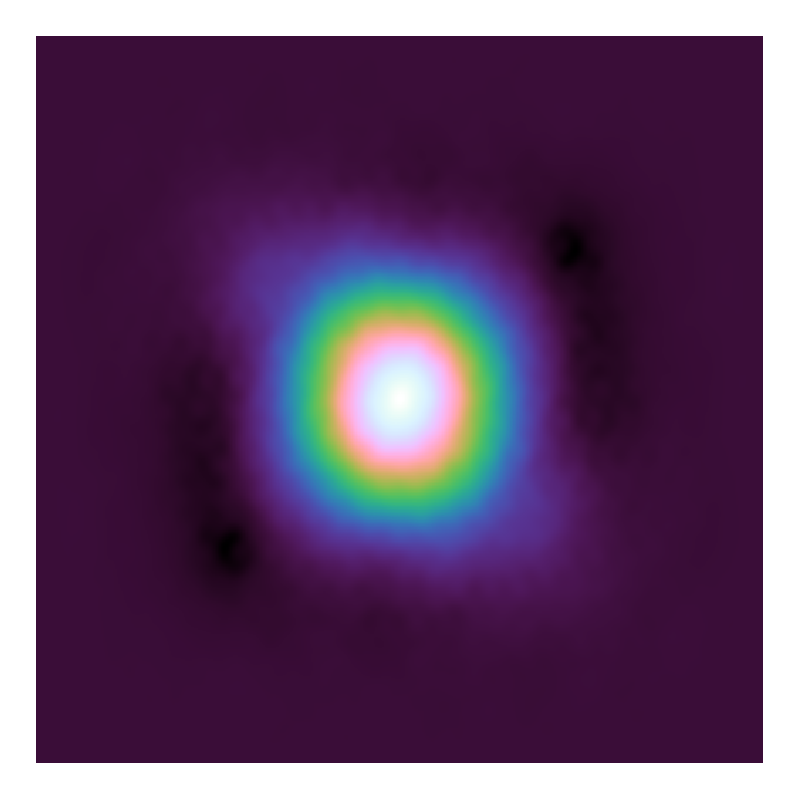
\includegraphics[width=\linewidth, clip, trim= 0.25in 0.25in 0.25in 0.25in]{./chapters/03.cd/simulated/psfSquared.png}
		\caption{Gradient update: $(PSF \star PSF)$.}
		\label{cd:efficient:update:psf}
	\end{subfigure}
	\caption{Example problem with two point sources.}
	\label{cd:efficient:update:figure}
\end{figure}

This means we can update the gradient map directly with the product of $(PSF \star PSF)$. We can simply shift $(PSF \star PSF)$ at the correct pixel location and subtract it from the gradient map directly. Although there is one issue: We use zero padded convolution. The $PSF$ at the edges of the image is masked. This means that the product $(PSF \star PSF)$ actually changes with the pixel location. If we update a pixel in the corner of the image, the actual update $(PSF \star PSF)$ at that location looks different than what was shown in Figure \ref{cd:efficient:update:psf}.

The exact update is again expensive to calculate. We need to shift the $PSF$ at its correct location and again calculate the correlation with itself. However, the exact gradient update only changes significantly at the edges of the image, when large parts of the $PSF$ are masked by the edges. Otherwise the difference between the exact update and simply shifting $(PSF \star PSF)$ at the pixel location is small. This is the reason why we chose to accept that the gradient update is only an approximation. The approximation only becomes inaccurate at the edges, and we use the algorithm in the Major cycle framework: Every Major cycle removes any inaccuracies we introduced during the previous cycle.  

\subsection{Efficient implementation pseudo-code}
Now we put all the run time improvements discussed before into the new implementation of the serial coordinate descent algorithm. We pre-calculate the Lipschitz constants and the gradient map. Then during iterations, we update the gradient map directly.

This leads to the following algorithm:
\begin{lstlisting}
dirty = IFFT(GridVisibilities(visibilities))
residualsPadded = ZeroPadding(dirty)

psfPadded = ZeroPadding(PSF)
psfPadded = FlipUD(FlipLR(psfPadded))
gradientUpdate = iFFT(FFT(ZeroPadding(PSF)) * FFT(psfPadded))

x = new Array[,]
gradientsMap = iFFT(FFT(residualsPadded) * FFT(psfPadded))
lipschitzMap = CalcLipschitz(PSF)

objectiveValue = 0.5* Sum(residuals * residuals) + ElasticNet(x)
maxAbsDiff = 0
do 
	oldObjectiveValue = objectiveValue
	
	//Step 1: Search pixel
	maxAbsDiff = 0
	maxDiff = 0
	pixelLocation = (-1, -1)
	for(i in Range(0, dirty.Length(0))
		for(j in Range(0, dirty.Length(1))
			oldValue = x[i, j]
			tmp = gradientsMap[i, j] + oldValue * lipschitzMap[i, j]
			optimalValue = Max(tmp - lambda*alpha) / (lipschitz[i, j] + (1 - alpha)*lambda)
			diff = optimalValue - oldValue
			
			if(maxAbsDiff < Abs(diff))
				maxAbsDiff = Abs(diff)
				maxDiff = diff
				pixelLocation = (i, j)
	
	//Step 2: Optimize pixel. Now all that is left is to add the maximum value at the correct location
	x[pixelLocation] += maxDiff
	
	//housekeeping
	shiftedUpdate = Shift(gradientUpdate, pixelLocation)
	gradientMap = gradientMap - shiftedUpdate * maxDiff
while epsilon < maxAbsDiff
\end{lstlisting}

In step 1, we replaced the gradient and Lipschitz calculation with lookups, reducing the runtime costs of the step. In this implementation, step 2 is trivial. We only need to update the reconstruction at the correct location. All the important work has already been completed in step 1.

The two most time consuming parts of this implementation are step 1, and updating the gradient map. Our implementation in .Net Core uses parallel computing for both parts. We search for the maximum pixel in parallel, and update the gradient map in parallel.


\subsection{Serial coordinate descent and similarities to the CLEAN algorithm}\label{cd:similarities}
When we look back at the CLEAN algorithm described in Section \ref{intro2:CLEAN}, we can see similarities in their structures: In the first step, CLEAN searches the location of the maximum pixel in the residuals, while serial coordinate descent searches the location of the absolute maximum change. In the second step, CLEAN subtracts a fraction of the $PSF$ at that location, while coordinate descent calculates the optimal pixel value and subtracts the product of $PSF \star PSF$ from the gradient map. 

CLEAN and serial coordinate descent have the same overall structure. But serial coordinate descent uses the gradient map instead of explicit residuals (the gradient map contains the information of the residuals implicitly). In a sense, the serial coordinate descent can be looked at as a CLEAN algorithm, which uses the gradient map instead of the residual map, and the product of $PSF \star PSF$ instead of the $PSF$. Both algorithms use essentially use the same operations, but the content in their memory is different. As such, one iteration of standard CLEAN is roughly as expensive as an iteration of serial coordinate descent. 

The side effect of their similar structure is that any speedup we achieve by using GPU acceleration for serial coordinate descent can plausibly be used to speedup CLEAN to a similar amount. Our distribution scheme for serial coordinate descent can also be used for a distributed standard CLEAN. 

The main difference between the two algorithms is that serial coordinate descent does not need the blurring step typically used in CLEAN algorithms. In Section \ref{intro2:CLEAN}, we introduced the CLEAN concept of the model image. Standard CLEAN detects point sources, and puts them in the model image. When the observation shows an extended emission, the standard CLEAN approximates it as a set of point sources. After CLEAN has finished finding all the point sources, it blurs the model image with the clean-beam, a 2d Gaussian representing the accuracy of the instrument, resulting in the reconstructed image.

In this project, we use the elastic net regularization, which has a simple model for extended emissions, namely the L2 norm. As such our serial coordinate descent algorithm can find the reconstructed image directly without any blurring. This may result in super-resolved reconstructions: The serial coordinate descent algorithm may find structures which are smaller than the accuracy limit of the instrument. We will show plausible super-resolved reconstructions by the serial coordinate descent algorithm with elastic net regularization in Section \ref{results}.

%Multi-scale CLEAN is what is used. Difficulty with MPI implementation because of a distributed convolution.

